The purpose of this experiment is to observe and study how validity cores evolves over unrolling the transition relation. It is interesting to see how quickly validity cores from a bounded proof converges to an actual minimal IVC.

\subsection{Experimental Setup}
  We perform our experiments on the same benchmark suite with 660 models introduced in Section \ref{sec:expsetup}. The experiment is conducted with a maximum depth of 10 and one hour timeout; i.e. for each model, if unrolling to depth 10 takes more than one hour, the \bvcalg algorithm will terminate. We capture $\bvc _{k}$ for $ 0 \leq k \le 10$. Then compare each $\bvc _{k}$ with each other to see how they alter during unrolling. Then, the final bounded validity cores obtained from at the maximum
  \footnote{Maximum in this experiment is 10. For most of the models, it is possible to reach this depth in less than an hour.}
  reachable depth in one hour, denoted by $\bvc _{max}$ , are considered as our final cores. These cores are compared with all the MIVCs gathered in Section \ref{subsec:res} to see if they match up with any of the actual minimal IVCs.

Research questions we would like to answer in this study are as follows:
\begin{itemize}
  \item \textbf{RQ1:} How many of the final BVCs do match up with one of the MIVCs? For how many of the models does the algorithm time out?
  \item \textbf{RQ2:} At what rate does size of the BVCs change? Does the size of the cores increase with the depth? 
  \item \textbf{RQ3:} How close is $\bvc _{max}$ to an actual MIVC? Is there any relationship with the size of the models and convergence of the BVCs?
\end{itemize}

\vspace{0.1in}
\subsubsection{RQ1}
The result of the experiments show that $\bvc _{max}$ is the same as one of the MIVCs for 474 models out of 660. For 27 of the models, $\bvc _{max}$ was not subset of any MIVCs (had additional elements, also none of the MIVCs was a subset of the $\bvc _{max}$). However, $\bvc _{max}$ was a subset of one of the MIVCs in 159 of the models.

We performed the experiments with \texttt{Z3} and \texttt{Yices} solvers. UNSAT core generation in \texttt{Z3} is faster, and \texttt{JKind} has special hack to get UNSAT cores from \texttt{Yices} because it does not have a support for it. Using \texttt{Z3}, 12 of the models did not reach depth 10 in one hour. With \texttt{Yices}, 18 of the models timed out. The interesting fact is that we had models that did not reach $\bvc _{10}$, but their $\bvc _{max}$ was the same as one of the MIVCs. For example, one of the models containing 571 design elements, only reached to $\bvc _{2}$, but $\bvc _{2}$ was the same as one of the MIVCs. 
BVC runs for that test case looks like as follows\footnote{This models is named ``steam\_boiler\_no\_arr1.lus'' in our benchmarks. You can see the results and model in our experimental directories \cite{expr}.}:

$|\bvc _{0}| = 6$, $|\bvc _{1}| = 11$, $|\bvc _{2}| = 128$ 

There are interesting case studies that from the beginning BVC was the same as one of the MIVCs. For example, in our benchmark we have a model with 27 design element\footnote{File ``car\_all\_e8\_856\_e2\_585.lus'' in our benchmark directory.}, for which $|\bvc _{i}| = 5$, $i \leq 0 \le 10$, and $\bvc _{0}$ is the same as its only one MIVC.

Note that the purpose of our experiments on BVCs and report such data is mostly to point out some research directions. Further studies may even can make use of BVCs in verification problems. A lot of time a valid property is hard or not inductive for the model checker to prove. In such cases, looking at the history of BVC runs may give us some confidence about the correctness of the property. The experimental results show that when we reach one of the actual MIVCs, BVC runs result in the same cores over and over. That is to say, when the BVC runs come to stable cores, it may imply we might have already seen all the reachable states, and implicitly known they are safe. Although this hypothesis may not be true and the reverse does not necessarily hold, it may be worth further investigations.

\vspace{0.1in}
\subsubsection{RQ2}
Our experimental results show that among 474 models for which $\bvc _{max}$ is the same as one of the MIVCs, the size of the BVCs were (nonstrictly) increasing 99.9\% of the time:
      $$ 0 \leq i \le max, |\bvc _{i}| \leq |\bvc _{i+1}|$$
      In other words, for only 12 of these models, the above relation did not hold.
      It is expected that bounded cores in each unrolling step (nonstrictly) increases as in each step more states are being reached and the cores required for the proof of the property is more likely to expand.
      We run the experiments over those 12 models with different solvers (once with \texttt{Z3} and once with \texttt{Yices}). In both runs, these models, mostly, behave the same (except 3 of them; see Table \ref{tab:bvc-abnormal}).

      It takes further study to see why those 12 models show different behavior, which is beyond the scope of this thesis. An initial explanation would be that when a model has several distinct MIVCs, the bounded core could change during unrolling. However, we examined these models and there are ones with a single MIVC that behaved abnormally. Another possibility could be that MIVCs obtained from \aivcalg ~contained timeout loops; i.e. we do not have the exact minimal IVCs for those cases (for example model\#6 in Table \ref{tab:bvc-abnormal}).

       The result of BVC runs for these models (on \texttt{Yices}) is shown in Table \ref{tab:bvc-abnormal}. 
       
       In order to show how quickly BVCs change and converge to an actual MIVC, we chose $\bvc _{0}$, $\bvc _{3}$, and $\bvc _{max}$  runs and plot the size of the cores. Mostly for models with less than 200 design elements, size of BVCs did not change much from depth 3 to 9. For the larger models there is some difference between the size of $\bvc _{3}$ and $\bvc _{max}$. Figure \ref{fig:bvc-growth} (a) shows a picture containing all the models. Figure  \ref{fig:bvc-growth} (b) is the enlarged version for some of the smaller models, and Figure  \ref{fig:bvc-growth} (c) magnifies the parts for larger models. 
       
 \begin{figure}
 \centering
  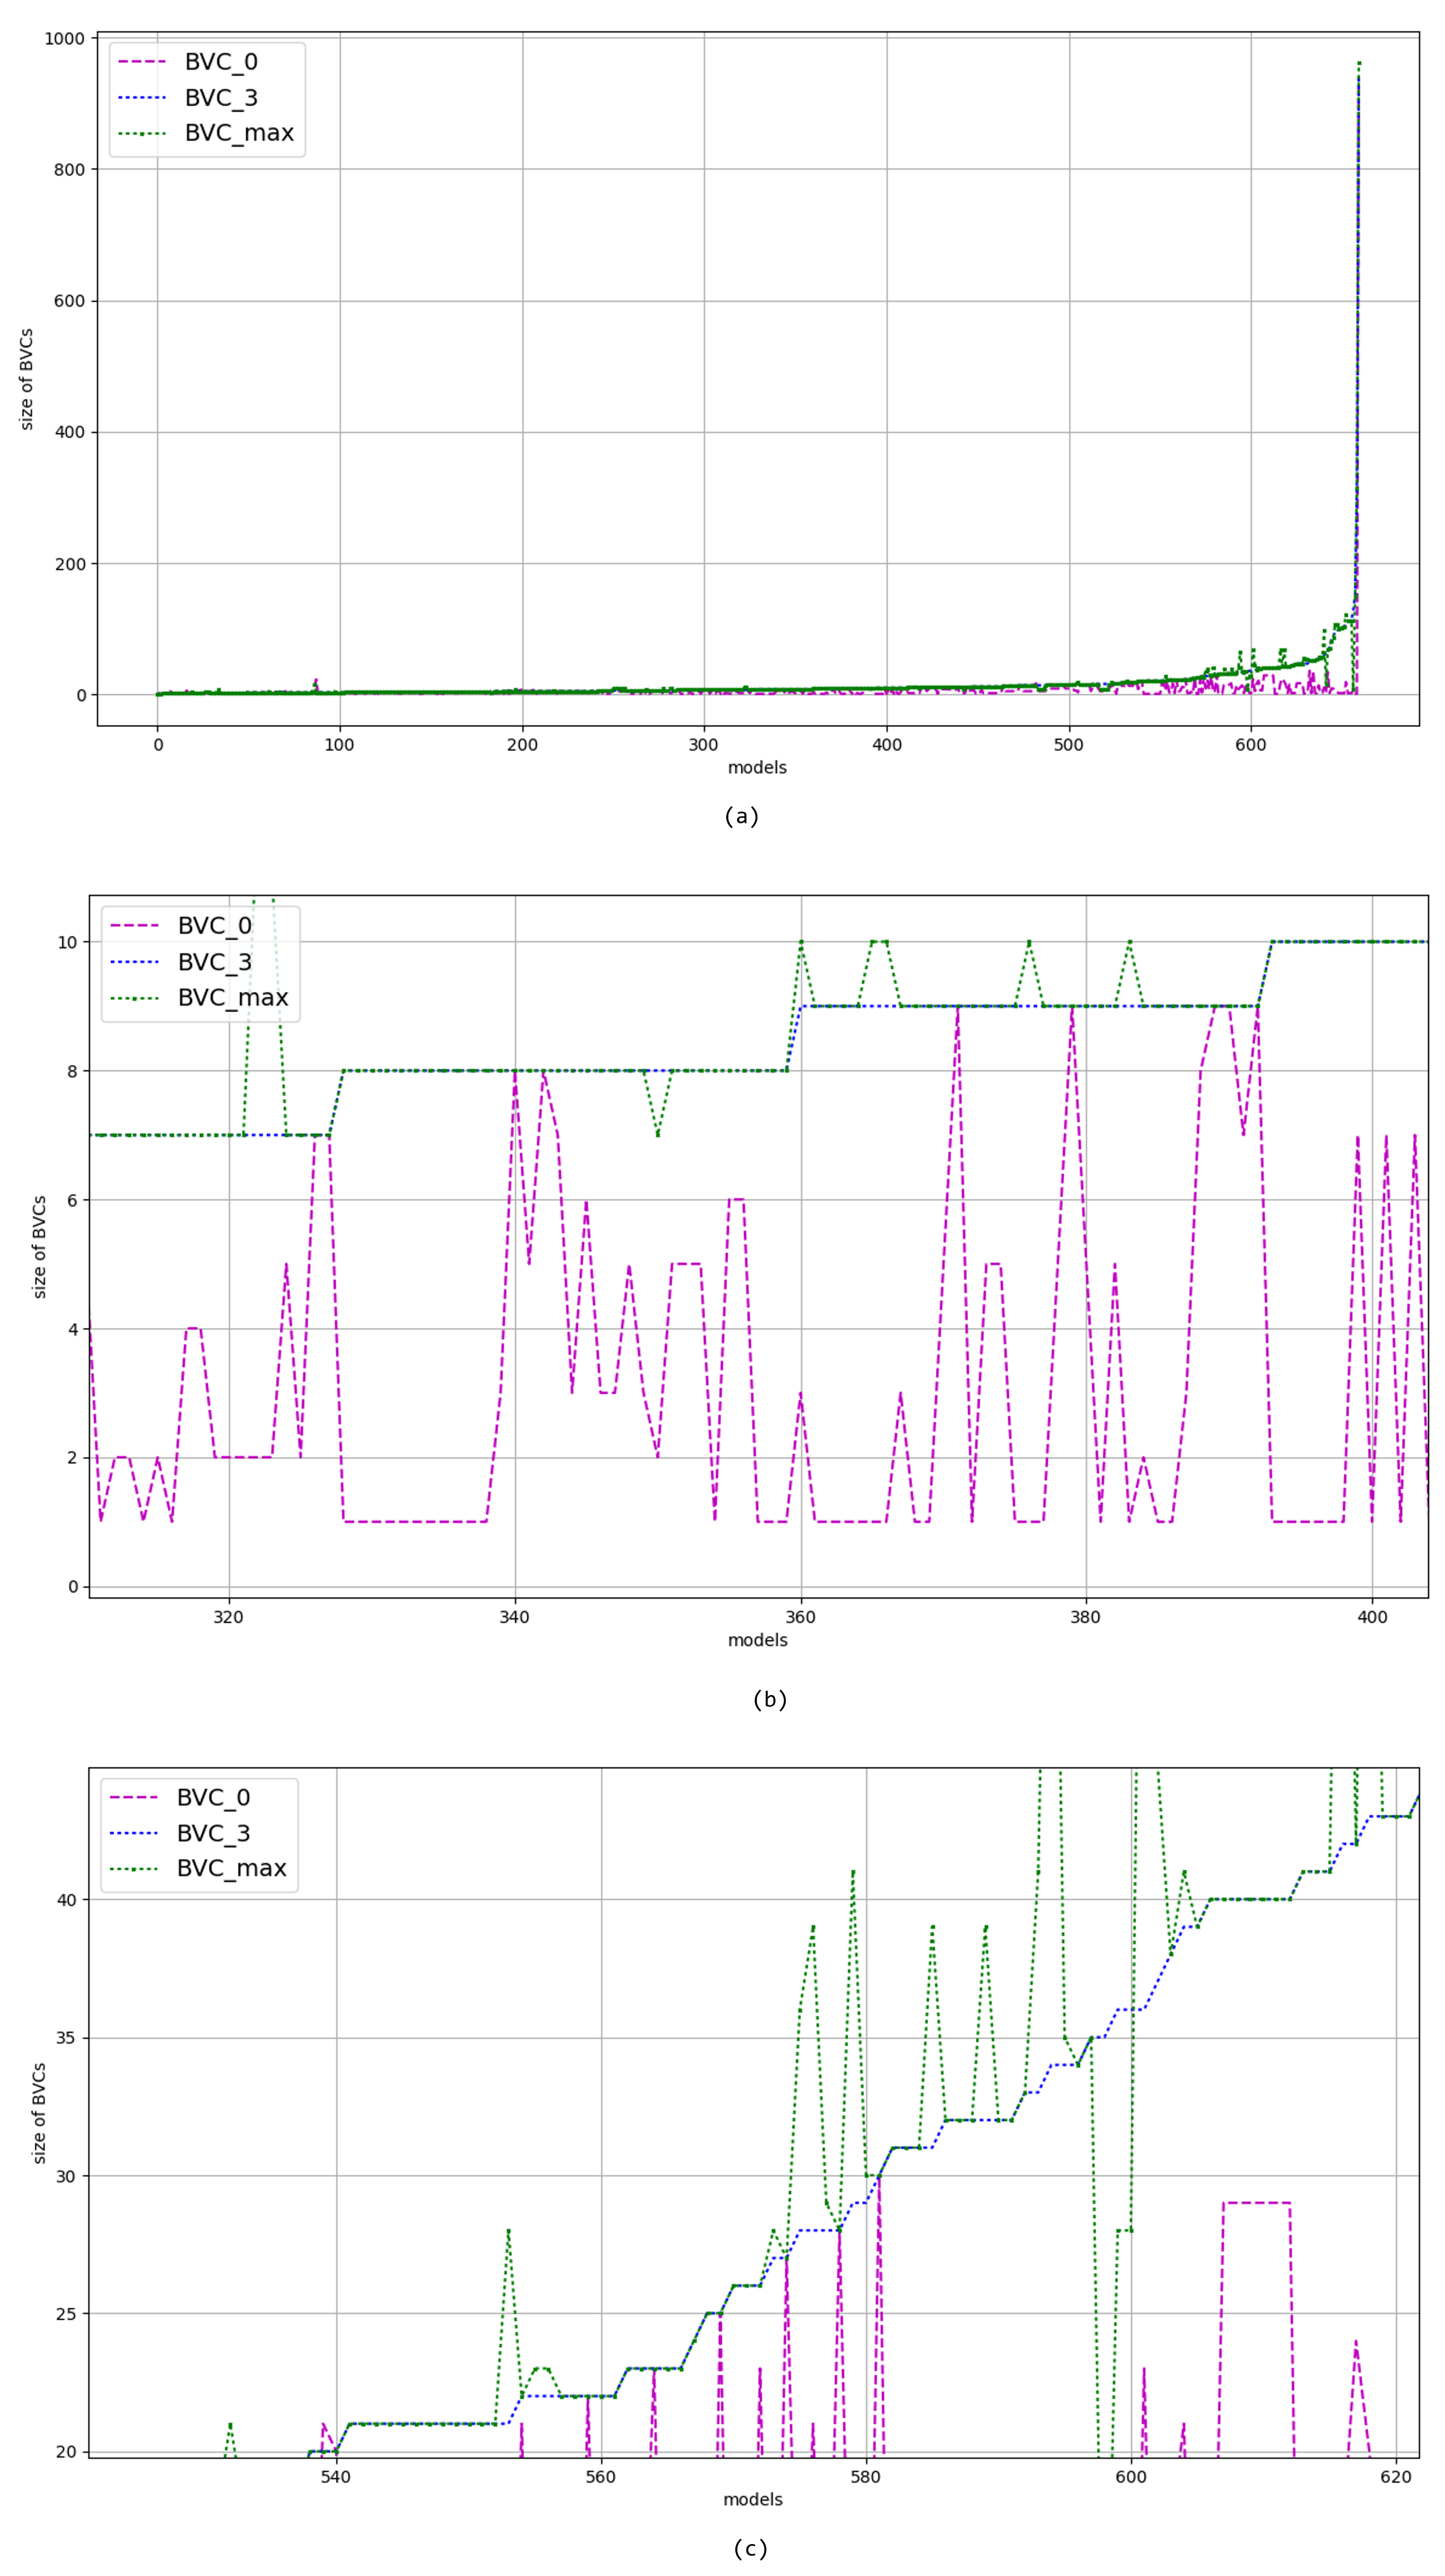
\includegraphics[width=.85\columnwidth]{figs/bvc_g.jpg}
  %\vspace{-0.1in}
  \caption{Size of BVCs at depth 0, 3, max}
  \vspace{0.1in}
  \label{fig:bvc-growth}
\end{figure}

       
       

\begin{table}
  \caption{BVC runs for the models with non-increasing behavior where $\bvc _{max}$ is the same as one of the MIVCs}
  \centering
  \begin{tabularx}{\linewidth}{ |c||c|c|c|c|c|c|c|c|c|c||L|L|}
    \hline
    $|\bvc _{i}|$ ~/~ $i=$ & 0 & 1 & 2 & 3 & 4 & 5 & 6 & 7 & 8 & 9 & \small{model size} & \small{\#of MIVCs} \\[0.5ex]
    \hline\hline
    
    model\#1& 2 & 9 & 34 & 36& 28 & 28 & 28 & 28 & 28 & 28 & 70&1 \\[0.5ex]
    model\#2& 5 & 15 & 11& 11& 11 & 11 & 11 & 11 & 11 & 11 & 123 &1\\[0.5ex]
    model\#3& 8 & 9& 13& 33& 28& 40& 38& 41& 41& 41&57 &7 \\[0.5ex]
    model\#4& 2& 5& 8& 10& 12& 10& 10& 10& 10& 10 &64 &9\\[0.5ex]
    \small{model\#5 (\texttt{Yices})}&9& 24 & 84& 84& 82& 82& 82& 82& 82& 82&96 &1\\[0.5ex]
    \small{model\#5 (\texttt{Z3})}& 9& 24& 82& 82& 82& 82& 82& 82& 82& 82&96 &1\\[0.5ex]
    model\#6& 5& 6& 5& 7& 5& 7& 5& 7& 5& 7& 7 &1\\[0.5ex]
    model\#7& 5& 6& 6& 5& 5& 6& 6& 5& 5& 6&6 &1\\[0.5ex]
    \small{model\#8 (\texttt{Yices})}& 9& 12& 14& 28& 37& 36& 36& 36& 36& 36&103&1 \\[0.5ex]
    \small{model\#8 (\texttt{Z3})}&9& 12& 14& 28& 37& 37& 37& 37& 37& 37& 103&1\\[0.5ex]
    \small{model\#9 (\texttt{Yices})}& 2& 6& 10& 4& 4& 4& 4& 4& 4& 4 &64&1 \\[0.5ex]
    \small{model\#9 (\texttt{Z3})}& 2& 4& 4& 4& 4& 4& 4& 4& 4& 4 &64&1\\[0.5ex]
    model\#10& 2& 6& 8& 11& 7& 7& 7& 7& 7& 7 &64&1\\[0.5ex]
    model\#11& 4& 13& 32& 47& 61& 54& 54& 54& 54& 54 &103&8 \\[0.5ex]
 \small{model\#12 (\texttt{Yices})}& 8& 8& 21& 29& 39& 38& 38& 40& 41& 41&57&6\\[0.5ex]
  \small{model\#12 (\texttt{Z3})}& 8& 17& 21& 29& 32& 38& 38& 32& 32& 32&57&6 \\[0.5ex]
    \hline
  \end{tabularx} \\
  \label{tab:bvc-abnormal}
\end{table}
      

\vspace{0.1in}
\subsubsection{RQ3}
We calculated the difference of $\bvc _{max}$ of each model with its MIVCs. Part of the results is described in \textbf{RQ1}. If $\bvc _{max}$  is the subset of one of the MIVCs, we calculated the difference between those two, and if not, $\bvc _{max}$  is compared with one of the MIVCs of the model, selected randomly.  Figure \ref{fig:dif-bvc} visualizes the results. Figure \ref{fig:bvc-size} shows the size of the models versus the differences line from Figure \ref{fig:dif-bvc} in logarithmic scale.

 \begin{figure}
 \centering
  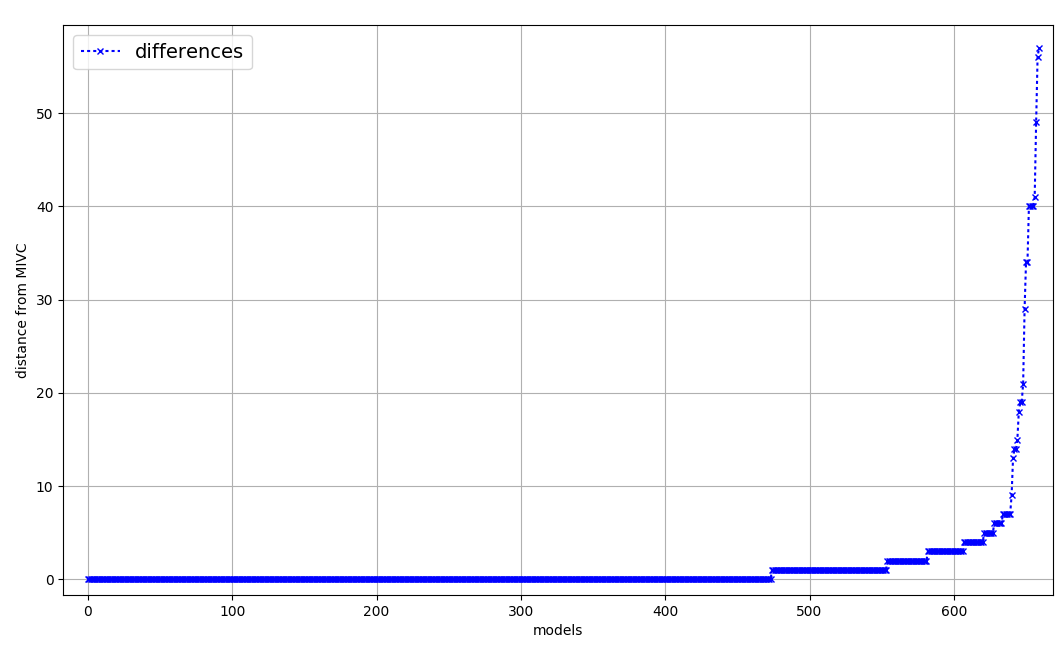
\includegraphics[width=\columnwidth]{figs/bvc_dif_yices.png}
  %\vspace{-0.1in}
  \caption{Difference between $\bvc _{max}$ and MIVCs}
  \vspace{0.1in}
  \label{fig:dif-bvc}
\end{figure}
 
 \begin{figure}
 \centering
  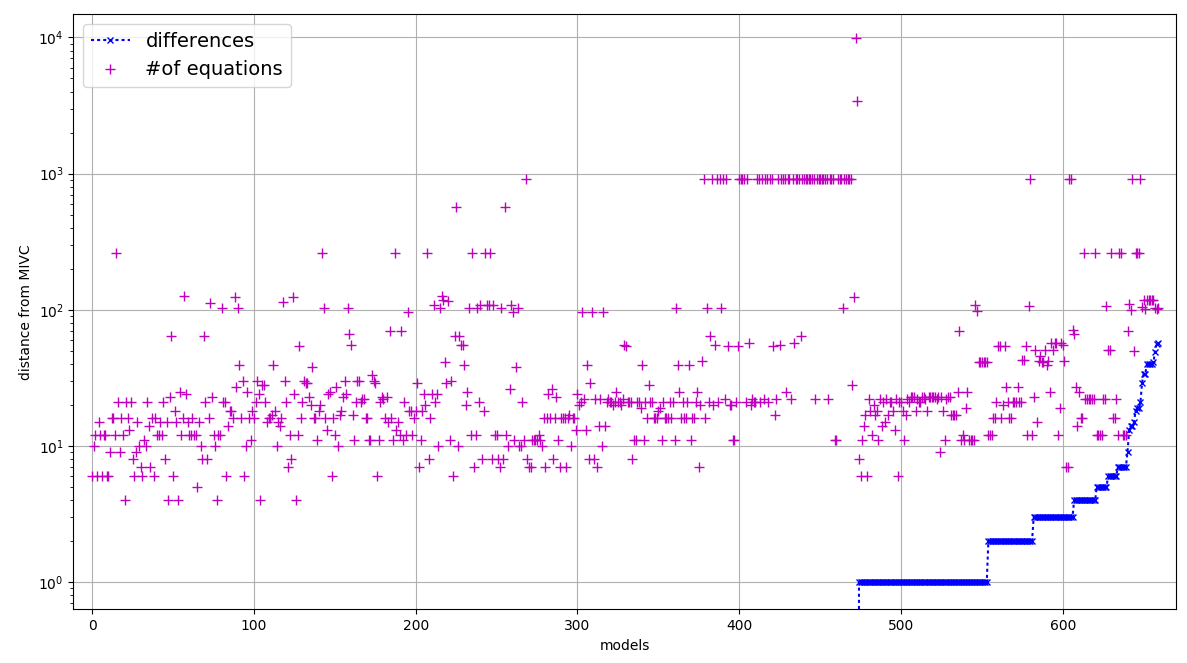
\includegraphics[width=\columnwidth]{figs/bvc_modelsize_yices.png}
  %\vspace{-0.1in}
  \caption{Difference between $\bvc _{max}$ and MIVCs vs the model size}
  \vspace{0.1in}
  \label{fig:bvc-size}
\end{figure} 